
%Prva naredba uvijek definira klasu dokumenta. Mi koristimo 'article'

\documentclass[a4paper,12pt,oneside]{article}




%***********************************************************************************
% Sada slijedi niz poziva Paketa funkcija cije ce se naredbe kasnije koristiti:
%***********************************************************************************

%Paket za upravljanje sa listama
\usepackage{enumitem}

% Paket za podesavanje brojeva stranica
\usepackage{scrlayer-scrpage}                  
	\ifoot[]{}
	\cfoot[]{}
	\ofoot[\pagemark]{\pagemark}
	\pagestyle{scrplain}
	
	
% Najcesce koristeni paketi za matematiku i formatiranje rada:
\usepackage{amsmath, amsthm}
\usepackage{mathtools}
\usepackage{latexsym,amsfonts,amssymb,amsbsy,graphics}
\usepackage{graphicx}
\usepackage[T1]{fontenc}
\usepackage[croatian]{babel} %Omogucava pisanje hrvatskih znakoba
\usepackage{gensymb}
\usepackage{pdfpages}  %Omogucava importiranje stranica pdf fila u dokument
\usepackage{pdflscape} %Omogucava okretanje pojedine stranice landscape dok su ostale portrait


% Paket za postavke naslova i podnaslova
\usepackage{titlesec}  
	\newcommand{\periodafter}[1]{#1.}
	\titleformat{\section}[hang]{\bf\large\uppercase}{\thesection.}{5pt}{}{}
	\titleformat{\subsection}[hang]{\bf\large}{\thesubsection.}{3pt}{}{}

% Dva paketa za imenovanje slika i tablica
\usepackage{subcaption}
\usepackage[labelfont=bf,textfont=it,labelsep = colon]{caption}  
	\captionsetup[figure]{name=SL.}
	\captionsetup[table]{name=Tab.}

% Paket sa bojama za formatiranje svega gdje se mjenja boja
\usepackage{xcolor}

% Paket za omogucavanje importiranja programskih kodova u tekst
\usepackage{listings} 
	\lstset{
  		numbers=left,
  		numberstyle=\tiny,
  		columns=fullflexible,
  		breaklines=true,
  		postbreak=\mbox{\textcolor{red}{$\hookrightarrow$}\space},
  		xleftmargin=5.0ex
	}
	\renewcommand{\lstlistingname}{Primjer koda}% Listing -> Algorithm

% Paket za formatiranje Sadrzaja
\usepackage[dotinlabels]{titletoc}
	\dottedcontents{section}[5em]{\bfseries}{2em}{1pc}
	\dottedcontents{subsection}[7em]{}{2em}{1pc}
	
	
	
% Najbolji paket u svemiru za matematicko pisanje tekstova
\usepackage{physics}

% Paket za postavljanje linkova na koje se moze klikat u pdfu (prema formuli broj x- click odvede na to)
\usepackage{hyperref}                 
\hypersetup{
    colorlinks,
    linkcolor={red!50!black},
    citecolor={blue!50!black},
    urlcolor={blue!80!black}
}


% Postavke margina stranica - NE DIRAJ

\setlength{\topmargin}{-0.7in}             
\setlength{\oddsidemargin}{-2mm}
\setlength{\evensidemargin}{-2mm}
\setlength{\textwidth}{170mm}
\setlength{\textheight}{256mm}
\setlength{\parindent}{1cm}


%**************************************************************************************************************
% Prostor za tvoje pakete je ovdje:
%**************************************************************************************************************

\usepackage[backend=biber, style=numeric]{biblatex}
\addbibresource{./supp_files/bibtex_baza.bib} 


% Paket za podršku za Unicode znakove s prelomom linije
\usepackage{newunicodechar}

% Definicija Unicode znakova s prelomom linije
\newunicodechar{́}{\nobreak\hspace{-1ex}\'{}} % U+0301
\newunicodechar{̌}{\nobreak\hspace{-1ex}\v{}} % U+030C

\usepackage{multicol}








%**************************************************************************************************************




%Kraj preamble naredbi, krece se sa pisanjem dokumenta
%**************************************************************************************************************


\begin{document}

%**************************************************************************************************************
% Postavke za numeriranje, prorede i ostalo
%**************************************************************************************************************

\setcounter{MaxMatrixCols}{20}                          %Postavka da matrica moze imati vise od 10 stupaca
\renewcommand{\baselinestretch}{1.5}                    %postavke za prored 1.5%
\renewcommand{\thefigure}{\thesection.\arabic{figure}}  %postavke za imenovanje slika po poglavljima%
\renewcommand{\thetable}{\thesection.\arabic{table}}   %postavke za imenovanje tablica po poglavljima%
\renewcommand{\theequation}{\thesection-\arabic{equation}} %postavke za brojanje jednadzbi po poglavljima%
\renewcommand{\refname}{LITERATURA}						% Uppercase Literatura

%**************************************************************************************************************




%**************************************************************************************************************
% NASLOVNA STRANICA
%**************************************************************************************************************

\begin{titlepage}

\begin{center}{\sc\Large sveu\v{c}ili\v{s}te josipa jurja strossmayera u osijeku}\\{\sc\Large fakultet elektrotehnike, ra\v{c}unarstva i informacijskih tehnologija osijek}\\
\bigskip

\vspace*{2cm}
{\large Sveučilišni studij}\\

\vspace*{7cm}

{\sc\LARGE Kontinuirana integracija primjenom dockera i gitlab pipelinea}

\vspace*{1cm}
{\large Diplomski rad}\\
\vspace*{3cm}
{\Large Valentin Loboda}\\
\vspace*{6cm}
{\normalsize Osijek, 2023.}
\end{center}

\end{titlepage}



%**************************************************************************************************************
% OBRASCI I FORMULARI
%**************************************************************************************************************

% Ubaciti pdf verzije D1 obrazca i izjave o originalnosti. 


%\newpage
%\includepdf{D1_obrazac.pdf}
%\newpage
%\includepdf{Originalnost.pdf}
%\newpage




%**************************************************************************************************************
% TABLE OF CONTENTS
%**************************************************************************************************************

{
	\hypersetup{linkcolor=black}
	\tableofcontents
}
%**************************************************************************************************************



\newpage
\section{Uvod}

U današnjem okruženju brzog razvoja softvera, ključno je usvojiti prakse koje osiguravaju učinkovitost, kvalitetu i pravovremenu isporuku softverskih rješanja. Kontinuirana integracija (CI) pojavila se kao temeljni koncept u ovom kontekstu. Automatizacijom procesa integriranja promjena koda, izvođenja testova i izgradnje artefakata, CI omogućuje razvojnim timovima otkrivanje i rješavanje problema rano u razvojnom ciklusu. To zauzvrat dovodi do poboljšane suradnje, smanjenih rizika i brže isporuke softvera.
Cilj ovog rada je istražiti i opisati koncept kontinuirane integracije na primjeru gitlab cjevovoda te istražiti alternativne platforme korištene za kontinuiranu integraciju. Ispitujući temeljna načela i najbolje prakse CIa, pružiti opće razumijevanje njegovih prednosti i izazova. gitlab cjevovod, često je korišten CI/CD alat koji omogućuje automatizaciju cijelog cjevovoda isporuke softvera, od upravljanja izvornim kodom, verzioniranja, testiranja do pokretanja aplikacije u oblaku, gdje je dostupna korisnicima.
Za prikaz rada gitlab cjevovod i uvid u implementaciju kontinuirane integracije, razvijena je web aplikacija u programskom jeziku java, koristeći spring boot okvir. Odabrana tema za aplikaciju je backend aplikacija za vođenje evidencije tarantula u hobiju teraristike, aplikacija korisnicima omogućuje upravljanje svojim terarijima, praćenje životnog ciklusa tarantula te vođenje evidencije hranjenja i ponašanja. Implementacijom kontinuirane integracije i gitlab cjevovoda u proces razvoja, cilj je prikazati prednosti ovih praksi u poboljšanju učinkovitosti, kvalitete i pouzdanosti životnog ciklusa razvoja softvera.

Rad je podijeljen u sedam poglavlja. Drugo poglavlje daje pregled kontinuirane integracije, uključujući njezinu definiciju, prednosti i izazove. Opisuje temeljna načela i najbolje prakse CIa, ističući njegovu ulogu u postizanju visokokvalitetnog razvoja softvera. U trećem poglavlju dan je uvid u različite platforme dostupne za implementaciju kontinuirane integracije. Ispitujući popularne CI/CD alate kao što su jenkins, travis CI i gitlab CI, uspoređene su njihove značajke, funkcionalnosti i mogućnosti integracije. Poglavlje četiri usredotočeno je na gitlab cjevovode, pružajući detaljan opis njegovih koncepata i kako ih učinkovito koristiti u CI/CD tijeku rada. Uz opis koncepata prikazan je tijek konfiguracije gitlab CI/CD cjevovoda na konkretnom primjeru, definirajući faze, poslove i tijekove rada. Nadalje, opisani su koraci integracije s docker hub repozitorijem kako bi se olakšao proces pokretanja aplikacije u oblaku.U petom poglavlju prikazana je implementacija web aplikacije koja koristi javu i okvir spring boot. Dan je pregled programskog jezika java i okvira spring boot. Uz opis prikazana je arhitektura i funkcionalnosti web aplikacije, ocrtavajući izbor dizajna i pristupe implementaciji. Uz implementaciju web aplikacije u ovom poglavlju pokrivena je i implementacija kontinuirane integracije i gitlab cjevovoda u proces razvoja. Postavljen je gitlab repozitorij za aplikaciju, definirana je CI/CD konfiguracija i uspostavljene su faze cjevovoda za verzioniranje, izgradnju, testiranje i pokretanje aplikacije u produkcijskoj okolini. Dodatno, istraženi su postupci automatiziranog testiranja i osiguranja kvalitete koda kako bi se osigurala robusnost i pouzdanost razvijene aplikacije. U sedmom poglavlju ocjenjeni su rezultati implementirane aplikacije, analizirajući učinkovitost kontinuirane integracije i gitlabovih cjevovoda u poboljšanju tijeka razvoja. Procjenjena je  izvedba i učinkovitost implementiranog sustava, ispitujući faktore kao što su vrijeme izrade, pokrivenost testom i stope uspješnosti implementacije.


\newpage

\section{Kontinuirana integracija}
Osobe koje nisu zaposlene u softverskim tvrtkama možda nisu svjesne sveobuhvatnog procesa uključenog u razvoj softvera izvan jednostavnog pisanja koda. Nakon što se kod pošalje na repozitorij, postoji dugačak i zamršen niz zadataka koji se moraju izvršiti da bi se izradio, potvrdio, osigurao, upakirao i implementirao softver prije nego što postane dostupan korisnicima. Ti se zadaci mogu izvršiti ručno ili, pod određenim okolnostima, u određenoj mjeri automatizirani. Međutim, i ručne i automatizirane metode pripreme softvera stvaraju određene izazove.

DevOps je nedavno nastala metodologija usmjerena na rješavanje ovih zadataka. Kombinira elemente automatizacije, suradnje, brze povratne informacije i iterativnog poboljšanja, omogućujući timovima da poboljšaju kvalitetu softvera, ubrzaju proces razvoja i smanje troškove\cite{cowell2023automating}. 
 
Rasprostranjena karakteristika brojnih softverskih projekata su produljena razdoblja tijekom razvoja u kojima aplikacija ostaje nefunkcionalna. Zapravo, značajan dio vremenskog okvira razvoja softvera koji su izradili veliki timovi provodi se u neupotrebljivom stanju. Temeljni razlog za ovaj fenomen sasvim je razumljiv: nema poticaja za pokušaj pokretanja cijele aplikacije dok se ona u potpunosti ne dovrši. Programeri doprinose promjenama i mogu provoditi automatizirana testiranja jedinica, ali se ne provode stvarno pokretanje i korištenje aplikacije u okruženju sličnom produkcijskom.

Ova je okolnost dodatno naglašena u projektima koji koriste proširene grane ili odgađaju testiranje prihvatljivosti za kasnije faze. U takvim projektima obično se značajne faze integracije vrše pred kraj razvojnog procesa, dajući razvojnom timu vremena da spoji grane i osigura da aplikacija funkcionira adekvatno za testiranje prihvaćanja. Da stvar bude složenija, određeni projekti nailaze na nesretnu spoznaju da njihov softver nije prikladan za namijenjenu svrhu tijekom integracijskog razdoblja. Ove faze integracije mogu postati iznimno dugotrajne, a što je najvažnije, njihovo trajanje ostaje nepredvidivo \cite{humble2010continuous}.

\subsection{Definicija kontinuirane integracije}
Koncept kontinuirane integracije prvi puta je predstavljen u knjizi Kenta Becka "Extreme Programming Explained", prvobitno objavljenoj 1999. Slijedeći načela ekstremnog programiranja, kontinuirana integracija proizašla je iz ideje da ako je redovita integracija baze koda korisna, zašto je ne učiniti stalnom praksom? U domeni integracije, "cijelo vrijeme" se odnosi na svaku instancu kada je izvršena bilo kakva izmjena u sustavu kontrole verzija.

Kontinuirana integracija označava značajan pomak u načinu razmišljanja. U nedostatku kontinuirane integracije, softver ostaje neispravan sve dok netko ne dokaže njegovu funkcionalnost, obično tijekom faza testiranja ili implementacije. Međutim, uz kontinuiranu integraciju, funkcionalnost softvera se provjerava (pod pretpostavkom prisutnosti odgovarajuće sveobuhvatnog paketa automatiziranih testova) sa svakom novom promjenom, a svi problemi se odmah identificiraju za trenutačnu verziju koda. Timovi koji učinkovito provode kontinuiranu integraciju mogu ubrzati isporuku softvera i naići na manje nedostataka u usporedbi s onima koji to ne čine. Otkrivanjem grešaka u ranoj fazi procesa isporuke, kada je manji trošak otkloniti ih, postižu se znatne uštede u pogledu vremena i troškova. Uslijed toga, kontinuiranu integraciju smatramo nezamjenjivom praksom za profesionalne timove \cite{humble2010continuous}.


\subsection{Izazovi implementacije kontinuirane integracije}
Kroz eksperimentalno istraživanje provedeno na Odjelu za računalne znanosti i inženjerstvo na Sveučilištu Chalmers u Göteborgu, Švedskoj, praćeno je sedam timova kroz 13 polu strukturiranih intervjua u periodu implementacije kontinuirane integracije u razvojni ciklus softvera unutar firme. Kroz provedeno istraživanje izazovi implementacije kontinuirane integracije podijeljeni su u sedam grupa prikazanih na slici \ref{f:izazovi implementacije kontinuirane integracije}


\begin{figure}[ht!] % [ht!] - opcija koja definira polozaj slike h-here, t-top, !-ne slusaj latexov AI. 
	\centering % - centrira sliku
	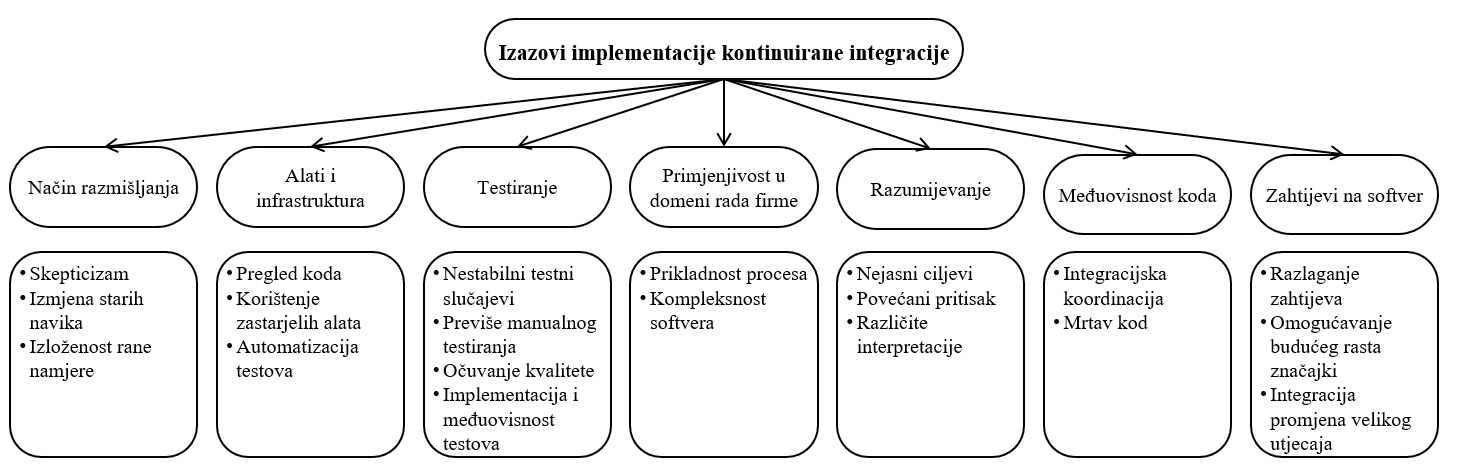
\includegraphics[scale=0.44]{./Slike/izazovi implementacije kontinuirane integracije.png} % [scale] - skalira dimenziju slike, moze i [width=0.6\linewidth] i slicno. 
	\caption{izazovi implementacije kontinuirane integracije \cite{challenges} \label{f:izazovi implementacije kontinuirane integracije}} % LABEL UVIJEK UNUTAR CAPTIONA. 
\end{figure}

\subsection{Proces kontinuirane integracije}
Tijekom faze kontinuirane integracije (CI), promjene razvojnog programera spajaju se i provjeravaju kako bi se osiguralo da kod ostaje funkcionalan. Glavni cilj CI-ja je brzo provjeriti te izmjene koda i odmah obavijestiti programera o svim problemima. Ovaj proces minimizira vrijeme tijekom kojeg je baza koda neupotrebljiva uslijed novo uvedenih pogrešaka. CI otkriva promjene koda i izvršava relevantne procese izgradnje kako bi pokazao da se promjene koda mogu uspješno izgraditi. Također može provoditi ciljane testove kako bi potvrdio da promjene koda rade neovisno, pri čemu ulazi proizvode željene izlaze i identificiraju i postupaju očekivano rukovajući pogrešnim ulazima.

Kontinuirana isporuka odnosi se na niz automatiziranih procesa, poznatih kao cjevovod, koji uključuje promjene koda i izvršava izgradnju, testiranje, pakiranje i povezane operacije za generiranje izdanja softvera koje se može koristiti. Općenito, to se postiže s malo ili nimalo ljudske intervencije.

Kontinuirana isporuka preuzima promjene koje je potvrdio i spojio CI i nastavlja s preostalim procesima u cjevovodu kako bi se proizveli željeni rezultati. Po izboru, može pokrenuti procese kontinuirane implementacije kako bi se izdanja automatski učinila dostupnima korisnicima. Mehanizam koji se koristi za kontinuiranu isporuku obično se naziva cjevovod kontinuirane isporuke, iako može imati i druga imena.

Iako krajnji rezultat cjevovoda često percipiramo kao ispravan kod ili softver koji se može koristiti, postoje ključni privremeni izlazi na putu. Zapravo, jedan od bitnih koraka u cjevovodu uključuje kombiniranje novopotvrđenih i spojenih promjena (iz CI-ja) s drugim kodom o kojem ovise ili s kojim trebaju raditi za generiranje artefakata. Upravljanje ovim srednjim rezultatima vrijedno je daljnjeg istraživanja.

Kontinuirano testiranje uključuje izvođenje automatiziranih testova ili drugih oblika analize koji se postupno šire kako kod napreduje kroz cjevovod kontinuirane isporuke. Neophodne su i preporučuju se različite vrste testiranja, uključujući:

\begin{itemize}
\item Unit testiranje, integrirano s procesima izgradnje tijekom CI faze, fokusira se na testiranje koda izolirano od drugog koda s kojim je u interakciji.
\item Integracijsko testiranje potvrđuje funkcioniranje grupa komponenti i usluga u kombinaciji.
\item Funkcionalno testiranje osigurava da izvršavanje funkcija u proizvodu daje očekivane rezultate.
\item Testiranje prihvatljivosti mjeri specifične karakteristike sustava prema unaprijed određenim kriterijima, kao što su performanse, skalabilnost, stres i kapacitet.
\end{itemize}

Mjerni podaci i analiza kodiranja ne spadaju u istu kategoriju kao testiranje prošao/nije prošao, ali doprinose kontinuiranom testiranju procjenom koda i kvalitete testiranja. Također se mogu koristiti kao kriteriji za pristupni (blokirajući ili dopuštajući) kod u različitim fazama cjevovoda. Neki primjeri ovih metrika i analiza uključuju:

\begin{itemize}
\item Analiza dijela koda pokrivenog testnim slučajevima, poznatog kao pokrivenost koda, koji se može mjeriti pomoću alata kao što je JaCoCo za Java kod.
\item Brojanje redaka koda, mjerenje složenosti i usporedba strukture i stila kodiranja s utvrđenim najboljim praksama, što se može postići pomoću alata kao što je SonarQube. Takvi alati provode provjere, uspoređuju rezultate sa željenim pragovima, kontroliraju daljnju obradu u cjevovodu i daju integrirana izvješća o ishodima.

\end{itemize}


Važno je napomenuti da nisu sve vrste testiranja prisutne u automatiziranom cjevovodu i mogu postojati nejasne granice između nekih od ovih kategorija testiranja. Međutim, krajnji cilj kontinuiranog testiranja unutar cjevovoda isporuke ostaje isti: postupno demonstrirati kroz testiranje i analizu da trenutna verzija koda zadovoljava potrebne standarde kvalitete.

Kontinuirana implementacija odnosi se na mogućnost preuzimanja izdanja koda koji je generirao cjevovod isporuke i automatskog stavljanja na raspolaganje krajnjim korisnicima. Ova vrsta cjevovoda često se naziva cjevovod za implementaciju. Proces implementacije može uključivati implementaciju u oblaku, ažuriranje web stranice, stavljanje ažuriranja na raspolaganje ili jednostavno ažuriranje popisa dostupnih izdanja, ovisno o tome kako bi korisnici "instalirali" softver.

Vrijedno je naglasiti da samo zato što se može postići kontinuirana implementacija ne znači da je svaki skup isporučenih rezultata iz cjevovoda uvijek implementiran ili da su nove funkcionalnosti odmah omogućene. Umjesto toga, cjevovod osigurava da je svaki skup isporučenih proizvoda dokazano sposoban za implementaciju kroz mehanizme poput kontinuiranog testiranja.

\begin{figure}[ht!] % [ht!] - opcija koja definira polozaj slike h-here, t-top, !-ne slusaj latexov AI. 
	\centering % - centrira sliku
	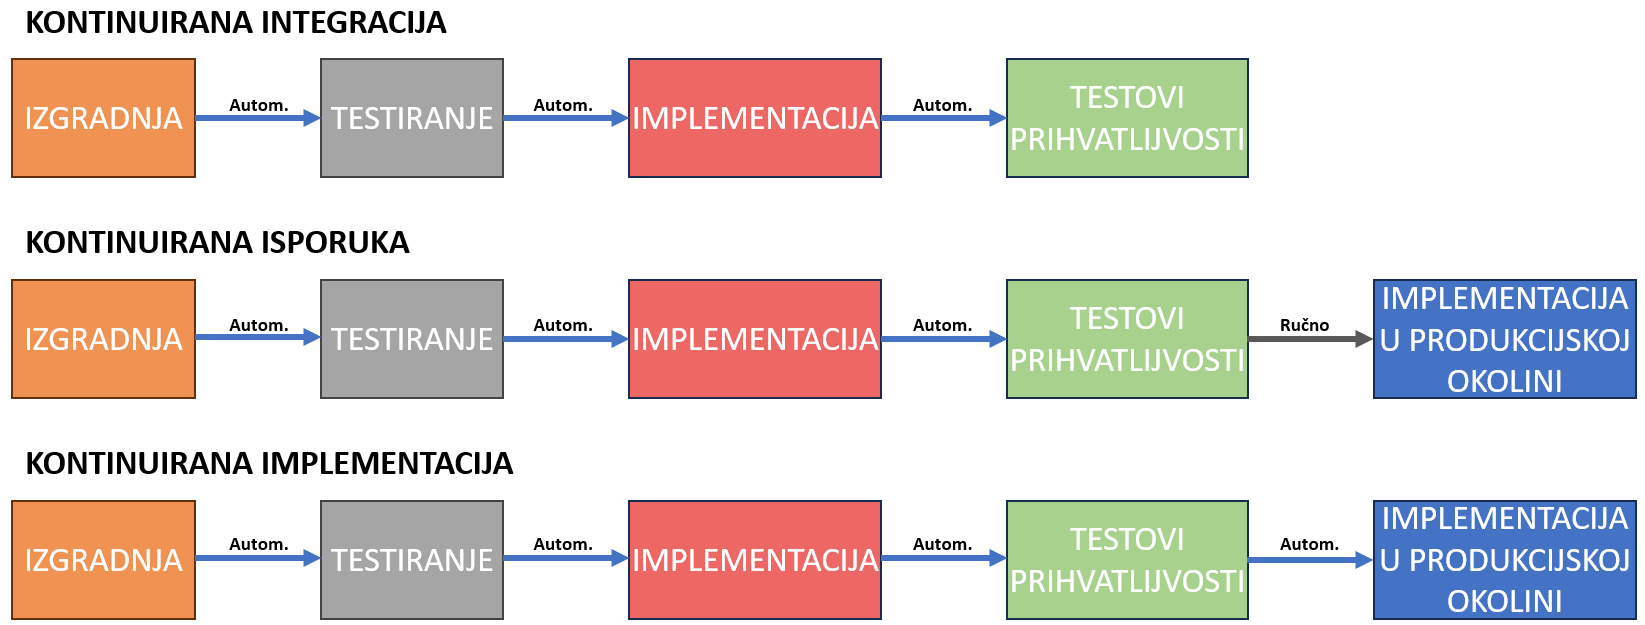
\includegraphics[scale=0.36]{./Slike/kontinuirana integracija, isporuka i implementacija.png} % [scale] - skalira dimenziju slike, moze i [width=0.6\linewidth] i slicno. 
	\caption{kontinuirana integracija, isporuka i implementacija \cite{ci_tools_slika} \label{f:kontinuirana integracija, isporuka i implementacija}} % LABEL UVIJEK UNUTAR CAPTIONA. 
\end{figure}

Vraćanje ili poništavanje implementacije za sve korisnike može biti skupa situacija, i tehnički i u smislu percepcije korisnika. Stoga odluka o tome treba li primijeniti oslobađanje iz cjevovoda može uključivati ljudsku prosudbu. Mogu se upotrijebiti različite metode za "testiranje" verzije aplikacije prije njegove potpune implementacije, stoga je preporuka da se posljednja verzija testira u integracijskoj okolini prije njezine implementacije za korisnike u produkcijsku okolinu. 
(Continuous Integration vs. Continuous Delivery vs. Continuous Deployment, 2nd Edition)

\newpage

\section{Platforme za provedbu kontinuirane integracije}

 Poduzeća sve više iskazuju afinitet prema DevOps metodologijama i agilnom pristupu razvoja softvera kako bi se ubrzao razvoj i isporuka kvalitetnih softverskih rješenja. Međutim, uspjeh ovog pristupa uvelike ovisi o odabiru pravih alata za kontinuiranu integraciju koji su usklađeni sa zahtjevima i potrebama poduzeća ili projekta.

Trenutačno je dostupan širok niz platformi za implementaciju kontinuirane integracije, što menadžerima predstavlja izazov pri odabiru najprikladnije za njihove projekte. Kako bi bili sigurni da je odabrana najbolja platforma, bitno je uzeti u obzir specifične tehničke karakteristike pojedine platforme.

Prvo, idealna platforma za kontinuiranu integraciju trebala bi ponuditi robustan ekosustav koji ubrzava isporuku projekta bez stvaranja zastoja. Osim toga, trebala bi se neprimjetno integrirati s uslugama u oblaku, omogućujući prijenos podataka u oblak i iz njega bez napora. Nadalje, platforma bi trebala pružiti pouzdane mogućnosti implementacije i podržavati integraciju s drugim alatima i uslugama koje se koriste u projektu. Ključno je dati prioritet sigurnosti, osiguravajući da odabrana CI platforma ne predstavlja rizik za podatke projekta, bez obzira na to radi li se o komercijalnom ili otvorenom programskom rješenju.

Osim tehničke sofisticiranosti, bitno je da se CI platforma uskladi s projektom i potrebama tvrtke. Ovisno o poslovnoj strategiji, moguće je odlučiti se za besplatni alat otvorenog koda ili komercijalno CI rješenje. Uz to, odabrana platforma trebala bi olakšati jednostavno upravljanje projektima i prijenos podataka, a istovremeno nuditi mogućnosti vizualizacije za bolje razumijevanje sadržaja.

Uzimajući u obzir tehničke aspekte i kompatibilnost s projektom i zahtjevima tvrtke, moguće je odabrati dobro zaokruženu CI platformu koja usmjerava razvojni proces i pridonosi cjelokupnom uspjehu projekta.

\newpage

\subsection{Pregled popularnih platformi}
Postoje brojne platforme za kontinuiranu integraciju no neke od najpopularnijih su:

\begin{multicols}{2}
\begin{itemize}
\item Gitlab CI
\item Jenkins
\item CircleCI
\item TeamCity
\item Bamboo
\item Travis CI
\item Buddy
\item Codeship
\item GoCD
\item Semaphore
\end{itemize}
\end{multicols}



\subsection{Karakteristike i funkcionalnosti platformi}
GitLab CI/CD, Jenkins, CircleCI, Travis CI i TeamCity neke su od najpopularnijih CI/CD platformi koje nude opsežnu podršku i integraciju za rad s Docker kontenjerima. Izbor između njih može ovisiti o čimbenicima kao što su specifični zahtjevi, preference alata i cjelokupni DevOps ekosustav u organizaciji. Činjenica da su ove platforme najpopularnije, ne znači da ostale platforme ne pružaju gotovo iste mogućnosti. U nastavku dan je pregled glavnih karakteristika i funkcionalnosti prethodno nabrojanih platformi.

\begin{enumerate}

\item 
Gitlab CI

GitLab je opsežan skup alata dizajniranih za nadgledanje različitih aspekata procesa razvoja softvera. U svojoj srži, GitLab je platforma temeljena na webu koja služi kao Git repozitorij, nudeći funkcionalnosti kao što su praćenje problema, analitika i Wiki za podršku kolaborativnom razvoju.

Jedna od bitnih značajki GitLaba je njegova sposobnost pokretanja izgradnje, izvršavanja testova i automatske implementacije koda sa svakom objavljenom promjenom. To znači da kad god se naprave promjene u bazi koda, GitLab može pokrenuti potrebne procese kako bi osigurao integritet i kvalitetu softvera. Ti se procesi mogu provesti unutar virtualnog stroja, Docker kontenjera ili na drugom poslužitelju, pružajući fleksibilnost i prilagodljivost razvojnom okruženju.

Neke od glavnih karakteristika su:
\begin{itemize}
\item GitLab je komercijalni alat i besplatni paket. Nudi hosting SaaS na GitLabu, na lokalnoj instanci i/ili u oblaku.
\item Učinkovito upravljajte pregledom, stvaranjem i upravljanjem kodom i projektnim podacima korištenjem alata za grananje.
\item Omogućuje brzu iteraciju i isporuku poslovnih vrijednosti kroz dizajn, razvoj i upravljanje kodom i projektnim podacima unutar objedinjenog distribuiranog sustava kontrole verzija.
\item Pouzdana i skalabilna platforma koja služi kao mjerodavan izvor za suradnju na projektima i kodu, osiguravajući jedinstveni izvor istine.
\item Olakšava usvajanje CI praksi od strane timova za isporuku kroz automatizaciju procesa izgradnje, integracije i verifikacije izvornog koda.
\item Omogućuje isporuku sigurnih aplikacija i usklađenost sa zahtjevima licenciranja pružanjem skeniranja repozitorija, testiranja sigurnosti statičke aplikacije (SAST), testiranja sigurnosti dinamičke aplikacije (DAST) i skeniranja ovisnosti.
\item Automatiziranje i pojednostavljeno izdavanje i isporuka aplikacija, smanjujući ručne napore i ubrzavajući proces implementacije.
\end{itemize}

\item 
Jenkins

Jenkins je besplatno dostupan poslužitelj za automatizaciju zadataka, poput izgradnje i kontinuirane integracije, u području razvoja softvera. Razvijen u Javi i sposoban za rad na različitim operativnim sustavima kao što su Windows, macOS i sustavima sličnim Unixu, Jenkins je opremljen širokim rasponom dodataka koji olakšavaju izgradnju, implementaciju i automatizaciju softverskih projekata.

Neke od glavnih karakteristika su:
\begin{itemize}
\item Jenkins je alat otvorenog koda s aktivnom zajednicom.
\item Jednostavna instalacija i nadogradnje na različitim operacijskim sustavima.
\item Sučelje je jednostavno i prilagođeno korisniku.
\item Jenkins se može proširiti velikom zbirkom dodataka koje je pridonijela zajednica.
\item Konfiguraciju okruženja lako je postaviti unutar korisničkog sučelja.
\item Jenkins podržava distribuiranu izgradnju kroz master-slave arhitekturu.
\item Rasporedi izrade mogu se prilagoditi na temelju izraza.
\item Podržava pokretanje shell i Windows naredbi u koracima prije izgradnje
\item Korisnici mogu primati obavijesti o statusu izgradnje.
\end{itemize}

\item 
CircleCI 

CircleCI je CI/CD alat koji olakšava brz razvoj i procese izdavanja softvera. Omogućuje automatizaciju u različitim fazama korisničkog cjevovoda, uključujući kompilaciju koda, testiranje i implementaciju.

Integracijom CircleCI-ja s platformama kao što su GitHub, GitHub Enterprise i Bitbucket, korisnici mogu pokrenuti izgradnju kad god se izvrše nove promjene koda. CircleCI nudi fleksibilnost hostinga kontinuirane integracije bilo u postavkama kojima upravlja oblak ili ih pokreće interno iza vatrozida na privatnoj infrastrukturi.

Neke od glavnih karakteristika su:
\begin{itemize}
\item Linux planovi počinju s opcijom pokretanja jednog posla bez paralelizma bez naknade. Projekti otvorenog koda dobivaju tri dodatna besplatna kontenjera. Tijekom prijave prikazane su cijene kako bi se korisnici odlučili koji plan(ove) trebaju.
\item Integracija je dostupna s Bitbucketom, GitHubom i GitHub Enterpriseom.
\item Izgradnje koda se mogu izvršiti pomoću kontenjera ili virtualnih strojeva.
\item Jednostavno otklanjanje pogrešaka.
\item Dostupne su mogućnosti automatizirane paralelizacije.
\item Brzi procesi testiranja.
\item Personalizirane obavijesti mogu se slati putem e-pošte i izravnih poruka.
\item Podržava kontinuiranu implementaciju, uključujući implementacije specifične za git grane.
\item Visoka razina prilagodbe.
\item Dostupno je automatsko spajanje i mogućnost izvršavanja prilagođenih naredbi za učitavanje paketa.
\item Proces postavljanja je brz i nema ograničenja u broju nadogradnji koje se mogu izvesti.
\end{itemize}

\item 
Travis CI

Travis CI je usluga specijalizirana za izgradnju i testiranje projekata kroz kontinuiranu integraciju. Integracijom s GitHub repozitorijem, Travis CI automatski identificira nove izmjene koda nakon čega pokreće izgradnju projekta i izvršava odgovarajuće testove i zadatke.

Travis CI nudi opsežnu podršku za različite konfiguracije izgradnje koda i programske jezike, uključujući, ali ne ograničavajući se na Node, PHP, Python, Javu i Perl.

Neke od glavnih karakteristika su:
\begin{itemize}
\item Travis CI je hosted CI/CD usluga. Privatni projekti mogu se testirati na travis-ci.com uz naknadu. Projekti otvorenog koda mogu se besplatno prijaviti na travis-ci.org
\item Proces postavljanja je brz i jednostavan.
\item Projekti na GitHub-a mogu se pratiti prikazom izgradnje uživo.
\item Podržani su zahtjevi za spajanje koda iz grane u granu.
\item Implementacija se može izvršiti na više usluga u oblaku.
\item Dostupne su unaprijed instalirane usluge baze podataka.
\item Automatske implementacije pokreću se nakon uspješne izgradnje koda.
\item Svaka izgradnja radi na čistom virtualnom računalu.
\item Podržava macOS, Linux i iOS platforme.
\item Podržano je više programskih jezika, uključujući Android, C, C\#, C++, Java, JavaScript (s Node.js), Perl, PHP, Python, R, Ruby i brojni drugi.
\end{itemize}

\item 
TeamCity

TeamCity, razvio je JetBrains, poslužitelj je za upravljanje izgradnjom i kontinuiranom integracijom. Služi kao vrijedan alat za izgradnju i implementaciju različitih vrsta projekata. TeamCity radi unutar Java okruženja i lako se integrira s Visual Studiom i ostalim IDE-ima. Ovaj svestrani alat može se instalirati na Windows i Linux poslužitelje, prilagođavajući se potrebama .NET i open-stack projekata.

U svojoj verziji 2019.1 TeamCity predstavlja novo korisničko sučelje zajedno s izvornom integracijom za GitLab. Također proširuje svoju podršku za GitLab i Bitbucket zahtjeve spajanja koda iz grane u granu. Osim toga, ovo izdanje uključuje značajke kao što su autentifikacija na temelju tokena, otkrivanje i izvješćivanje o Go testovima, kao i mogućnost rukovanja zahtjevima na AWS Spot Fleet.

Neke od glavnih karakteristika su:
\begin{itemize}
\item TeamCity je komercijalni alat s besplatnim i vlasničkim licencama.
\item Nudi različite metode za primjenu postavki i konfiguracija nadređenog projekta na podprojekte, promičući ponovnu upotrebu.
\item Podržava paralelne izgradnje koda u više okruženja, omogućujući istovremeno izvođenje.
\item Omogućuje značajke kao što su pregled izvješća o povijesti testiranja, prikvačivanje, označavanje i dodavanje međuverzija u favorite za učinkovito praćenje i upravljanje povijesti verzija.
\item Poslužitelj je visoko prilagodljiv, interaktivan i proširiv, što omogućuje prilagođene konfiguracije.
\item Osigurava funkcionalnost i stabilnost CI poslužitelja, promičući neometan rad.
\item Nudi fleksibilno upravljanje korisnicima, omogućava dodjelu korisničkih uloga, grupiranje korisnika, višestruke metode provjere autentičnosti i održavanje dnevnika radnji korisnika za transparentno praćenje aktivnosti poslužitelja.
\end{itemize}

\end{enumerate}

\subsection{Odabir najprikladnije platforme za implementaciju}

Pri odabiru platforme za implementaciju kontinuirane integracije, za aplikaciju implementiranu u sklopu ovoga rada, Jenkins i Gitlab platforme su bile glavni kandidati. I Jenkins i GitLab nude vrijedne značajke u svojim domenama. Jenkins pruža opsežnu jezičnu podršku i može se pohvaliti golemom bibliotekom dodataka. Njegovo korisničko sučelje pojednostavljuje zadatke kao što su postavljanje čvora, otklanjanje pogrešaka pokretača i implementacija koda. Alat je vrlo prilagodljiv, što omogućuje fleksibilno uređivanje konfiguracije. Budući da se samostalno hosta, Jenkins korisnicima pruža veću kontrolu nad radnim prostorima te je upravljanje pristupom jednostavno.
Međutim, Jenkins zaostaje kada je u pitanju analitika praćenja cjevovoda, što može biti nedostatak. Osim toga, konfiguriranje integracije dodataka i postavljanje alata može oduzimati puno vremena, otežavajući proces implementacije kontinuirane integracije.

S druge strane, GitLab služi kao sveobuhvatan DevOps alat koji obrađuje različite razvojne zadatke. Dolazi opremljen ugrađenim Git sustavom za kontrolu verzija, što olakšava integraciju s drugim rješenjima.

Jedna značajka GitLaba vrijedna pažnje je njegova sposobnost pružanja poslovnih uvida, nudeći jasnu vidljivost utjecaja promjena na performanse proizvoda. Statistika korisnika pomaže u praćenju korištenja resursa i optimizaciji procesa, no ova je značajka dostupna samo korisnicima koji plaćaju za Gitlab CI usluge. Praćenje problema je još jedna vitalna sposobnost, podržana značajkama kao što su rasprave u nitima, oznake i popisi zadataka, omogućujući učinkovito praćenje i dodjelu problema za brzo rješavanje. GitLab također omogućuje uvoz zadataka iz JIRA-e. Upravljanje spajanjem koda iz grane u granu olakšava suradnju i kontrolu verzija projekata.

GitLab se ističe u omogućavanju paralelnog izvođenja kroz faze, pojednostavljujući skaliranje pokretača. Dodavanje poslova i rješavanje konflikta u kodu je vrlo jednostavno. Alat daje prioritet sigurnosti projekta s odgovarajućim pravilima o privatnosti i neprimjetno se integrira s Dockerom.

S negativne strane, GitLab uvodi neke složenosti i napor, jer definiranje i rukovanje artefaktima za svaki posao postaje neophodno. Testiranje spojenog stanja iz grane u granu zahtijeva da se stvarno spajanje dovrši prije, stoga je bitno da razvojni programeri prije spajanja svog koda u main granu, spoje grane lokalno i tako spojen kod pošalju na git.

Iako GitLab uvodi neke složenosti, poput definiranja i rukovanja artefaktima za svaki posao, njegove sveobuhvatne značajke i mogućnosti integracije s docker registrima čine ga prikladnijim za kreiranu aplikaciju. Naravno, to ne znači da je Jenkins ili bilo koja druga platforma lošiji odabir, veliku ulogu u odabiru imala je i upoznatost s Gitlab cjevovodima kroz prijašnji rad i iskustvo.


\section{Gitlab pipeline koncepti i primjena}

Cjevovodi se najjednostavnije mogu objasniti kao niz automatiziranih shell naredbi, minimizirajući potrebu za ljudskim sudjelovanjem. Razumijevanje ovog temeljnog koncepta ključno je za razumijevanje CI/CD cjevovoda. Drugim riječima, CI/CD cjevovod može se opisati kao lanac naredbi koje izvršava robot i koje obuhvaćaju zadatke povezane s izgradnjom softvera, testiranjem i implementacijom.

Izvršenje ovih naredbi provode GitLab Runneri, robotski entiteti u procesu. Iz tehničke perspektive, GitLab Runner je kompaktni program koji prima naredbe od GitLab instance i izvršava ih u skladu s tim. Moguće je koristiti besplatni, zadani Gitlab runner koji nije potrebno dodatno konfigurirati, no također je moguća instalacija vlastite instance Gitlab runnera na virtualnom stroju.

Svaki put kada se cjevovod projekta izvede, on radi na određenoj verziji datoteka projekta. To implicira da se tijekom CI faze cjevovoda automatizirani testovi i skeniranja provode na jednoj verziji datoteka. Nakon toga, u fazi CD-a, ista verzija datoteka se postavlja u odgovarajuće okruženje. Ovaj se koncept također može izraziti kao cjevovod koji radi "protiv" određene verzije datoteka projekta.

Svrha cjevovoda je procijeniti stanje koda i implementirati ga kad god se naprave promjene. Posljedično, pokretanje cjevovoda projekta na kodu od prethodnog dana dalo bi poseban skup rezultata u usporedbi s pokretanjem s kodom iz tekućeg dana, čak i ako se cjevovod sastoji od identičnih faza, poslova i naredbi. Razlika u rezultatima nastaje zbog mogućih čimbenika kao što je dodavanje novih automatiziranih testova, uvođenje softverskih grešaka koje dovode do neuspjeha testa ili uključivanje ovisnosti sa sigurnosnim propustima. Imajući to u vidu, dva pokretanja cjevovoda generirala bi suprotne ocjene u pogledu kvalitete koda.

\subsection{Faze i zadatci u gitlab pipelineu}
Svaki cjevovod se sastoji od jedne ili više faza, koje su skupine povezanih zadataka. Tri najčešće korištene faze su sljedeće:
\begin{enumerate}
\item Izgradnja: Ova faza sadrži zadatke koji kompiliraju i pakiraju izvorni kod u format koji se može primijeniti.

\item Testiranje: Ova faza obuhvaća zadatke koji izvršavaju automatizirane testove, skeniranje kvalitete koda, linting i potencijalno sigurnosno skeniranje.

\item Implementacija: Ova faza je odgovorna za slanje koda u odgovarajuće okruženje na temelju Git grane ili oznake prema kojoj se cjevovod pokreće. 
\end{enumerate}

Ove tri faze unaprijed su konfigurirane u GitLabovim zadanim postavkama cjevovoda. Međutim, gitlab pruža fleksibilnost mijenjanja ove zadane konfiguracije dodavanjem, uklanjanjem ili zamjenom faza. Bez obzira na odabrane faze, preporuka je da ih se eksplicitno definira, čak i ako je krajnja odluka korištenje zadane tri faze. Iako se ovo može činiti opširnim, poboljšava čitljivost, pomaže u rješavanju problema i sprječava zabune u budućnosti.

Ne postoji ograničenje broja faza koje je moguće definirati. Čak i za vrlo jednostavne projekte, možemo stvoriti pojednostavljeni cjevovod sa samo jednom fazom. Imena faza mogu se birati slobodno, dopuštajući razmake i razne interpunkcijske simbole. Kako bi se osigurala čitljivost, predlaže se da imena faza budu što  sažetija, bez žrtvovanja jasnoće, jer duga imena mogu biti skraćena u GitLabovom grafičkom korisničkom sučelju.

Važno je napomenuti da GitLab ne provjerava tematsku vezu između zadataka unutar faze; ova odgovornost leži na osobi koja ih implementira. Posljedično, postoji sloboda kreiranja neorganiziranog i neorganiziranog cjevovoda. Na primjer, moguće je pokrenuti automatizirane regresijske testove u fazi pod nazivom "Primjena dokumentacije" ili implementirati dokumentaciju u fazi pod nazivom "priprema-testnog okruženja". Podjela cjevododa u faze i dodjela zadataka svakoj fazi u potpunosti je na osobi koja vrši implementaciju. Smatra se najboljom praksom povremeno pregledavanje i refaktoriranje strukture cjevovoda kako bi se osigurala jasnoća i dosljednost.


Kada su u pitanju komponente GitLab CI/CD cjevovoda, poslovi se mogu promatrati kao sljedeća razina ispod faza. Svaki stupanj sadrži jedan ili više poslova, a svaki posao pripada određenom stupnju.

\begin{figure}[ht!] % [ht!] - opcija koja definira polozaj slike h-here, t-top, !-ne slusaj latexov AI. 
	\centering % - centrira sliku
	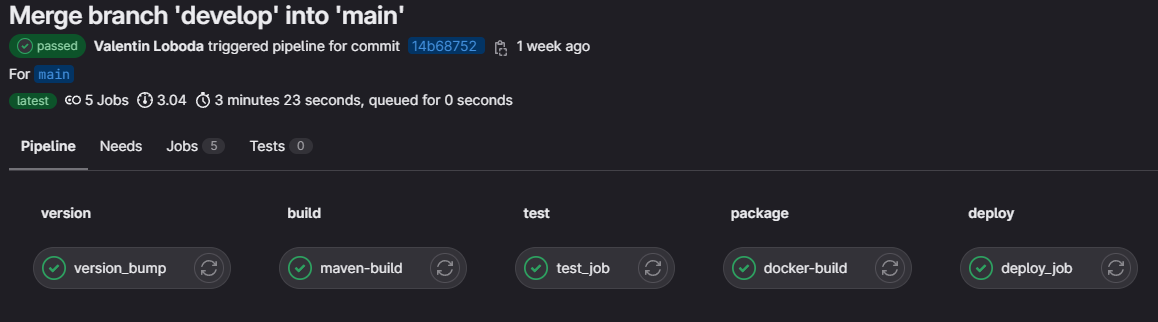
\includegraphics[scale=0.5]{./Slike/gitlab ci job overview main branch.png} % [scale] - skalira dimenziju slike, moze i [width=0.6\linewidth] i slicno. 
	\caption{prikaz Gitlab posla s pripadajućim fazama (placeholder slika) \label{f:prikaz Gitlab posla s pripadajućim fazama}} % LABEL UVIJEK UNUTAR CAPTIONA. 
\end{figure}

Gledajući sliku zaslona \ref{f:prikaz Gitlab posla s pripadajućim fazama}, možemo uočiti da faza izgradnje uključuje posao pod nazivom build-job, faza testiranja uključuje posao pod nazivom test-job, a faza Deploy uključuje posao pod nazivom deploy-job.

Kao što pokazuju ovi nazivi poslova, obično je svaki posao odgovoran za obavljanje određenog zadatka. Na primjer, posao bi mogao kompajlirati Java izvorni kod u klase, drugi posao bi mogao resetirati podatke testne baze podataka, a još jedan posao bi mogao gurnuti Docker sliku u registar. Međutim, baš kao što GitLab ne provodi tematsku sličnost poslova unutar faza, također ne potvrđuje ispunjavaju li poslovi stvarno zadatak koji sugeriraju njihova imena. Drugim riječima, imate slobodu kreirati posao pod nazivom compile-java koji briše zalutale datoteke generirane automatiziranim testovima ili posao pod nazivom deploy-to-production koji pokreće sigurnosni skener. Stoga je važno biti oprezan i promišljen pri imenovanju svojih poslova, povremeno ih pregledavajući kako biste osigurali točnost i čitljivost.

Osim toga, GitLab ne nameće zahtjev da svaki posao obavlja samo jedan zadatak. To znači da vas ništa ne sprječava da napravite posao pod nazivom test koji izvršava višestruke automatizirane pakete testova, testove performansi i sigurnosne skenere. Međutim, smatra se najboljom praksom svaki posao fokusirati na jedan zadatak. GitLab vam omogućuje kreiranje poslova s različitim opsegom, širokim ili uskim, u skladu s vašim specifičnim potrebama.


\subsection{Definiranje gitlab CI/CD konfiguracije}

U poglavlju iznad definiran je proces konfiguriranja CI/CD cjevovoda, koji uključuje definiranje faza, poslova i naredbi, no kako zapravo izvesti ovu konfiguraciju i gdje? Sva konfiguracija za CI/CD cjevovod obavlja se unutar datoteke pod nazivom .gitlab-ci.yml, koja se nalazi u korijenskom direktoriju repozitorija projekta. Ako istražimo bilo koji javni GitLab projekt s implementiranim cjevovodom, možemo pronaći datoteku s ovim nazivom koja određuje radnje konfigurirane za taj projekt.

Svaka datoteka .gitlab-ci.yml koristi jezik YAML(yet another markup language ili YAML ain't markup language) dizajniran za tu svrhu. Ovaj se jezik sastoji od ključnih riječi, vrijednosti i nekih sintaktičkih elemenata. Određene ključne riječi koriste se za definiranje faza i poslova unutar tih faza. Ostale ključne riječi koriste se za prilagodbu poslova i njihovog ponašanja unutar cjevovoda. Dodatno, postoje ključne riječi za postavljanje varijabli, određivanje Docker slika za poslove i utjecaj na cjelokupni cjevovod na različite načine. Ovaj jezik je dovoljno fleksibilan da se prilagodi širokom rasponu zadataka u CI/CD cjevovodima, ali ipak nije pretjerano složen (barem nakon što se stekne neko iskustvo u pisanju i razumijevanju ovih CI/CD konfiguracijskih datoteka).

Postoji otprilike 30 ključnih riječi dostupnih za korištenje u datoteci .gitlab-ci.yml. Umjesto pamćenja svih pojedinosti i opcija konfiguracije povezane sa svakom ključnom riječi, preporuča se usredotočavanje na shvaćanje ukupnih mogućnosti koje nude CI/CD cjevovodi. Nakon shvaćanja općih mogućnosti, lakše je upoznati se sa specifičnim ključnim riječima prema potrebi. Službena dokumentacija GitLaba najpouzdaniji je izvor informacija o ključnim riječima, osobito jer se one mogu mijenjati tijekom vremena.

\subsection{Docker i povezivanje s dockerom za kontejnerizaciju aplikacije}

Docker ekosustav potaknuo je uspješnu zajednicu koja se sastoji od programera i administratora sustava. Slično pokretu DevOps, ova je zajednica prepoznala vrijednost rješavanja operativnih izazova putem koda, što je dovelo do razvoja poboljšanih alata. U slučajevima kada Dockerov izvorni alat zakaže, razne tvrtke i pojedinci su preuzeli inicijativu da popune te nedostatke pa tako primjerice Gitlab ima dostupan vlastiti Docker registar u koji se mogu spremati kontenjerizirane verzije aplikacije. Mnogi Docker alati su otvorenog koda, što omogućuje njihovo proširenje i prilagodbu drugim organizacijama kako bi zadovoljile svoje specifične zahtjeve. 

Docker se može podijeliti u dvije glavne komponente: klijent i poslužitelj/daemon. Dodatno, postoji izborna treća komponenta koja se zove registar, koja služi kao pohrana Docker slika i njihovih metapodataka. Poslužitelj/daemon odgovoran je za kontinuirane zadatke izgradnje, pokretanja i upravljanja spremnicima, dok se klijent koristi za davanje uputa poslužitelju o radnjama koje treba izvršiti. Docker demon se može instalirati na više poslužitelja unutar infrastrukture, a jedan klijent može komunicirati s više poslužitelja. Klijenti djeluju kao glavni pokretači komunikacije, ali Docker poslužitelji također mogu izravno komunicirati s registrima slika prema uputama klijenta. U tom kontekstu, klijenti su odgovorni za izdavanje uputa poslužiteljima, dok su poslužitelji prvenstveno usredotočeni na hosting i upravljanje kontejnerskim aplikacijama.

\begin{figure}[ht!] % [ht!] - opcija koja definira polozaj slike h-here, t-top, !-ne slusaj latexov AI. 
	\centering % - centrira sliku
	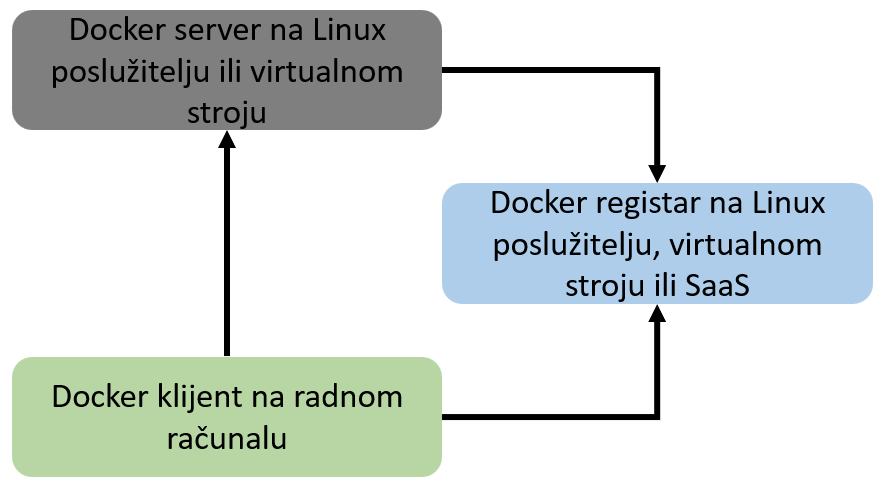
\includegraphics[scale=0.5]{./Slike/docker klijent-server model.png} % [scale] - skalira dimenziju slike, moze i [width=0.6\linewidth] i slicno. 
	\caption{Docker klijent/server model \cite{kane2023docker} \label{f:docker klijent/server model}} % LABEL UVIJEK UNUTAR CAPTIONA. 
\end{figure}

Docker ima jedinstvenu strukturu u usporedbi s nekim drugim klijent/poslužitelj softverima. Sastoji se od docker klijenta i dockerd poslužitelja. Međutim, umjesto da bude potpuno monolitan, poslužitelj koordinira razne druge komponente u pozadini u ime klijenta. Jedna od tih komponenti je containerd-shim-runc-v2, koja olakšava interakciju s runc i containerd. Unatoč ovim temeljnim složenostima, Docker pojednostavljuje proces pružanjem jednostavnog sučelja klijenta i poslužitelja. U većini slučajeva može ga se shvatiti kao jednostavnog klijenta i poslužitelja. Tipično, svaki Docker host pokreće jedan Docker poslužitelj koji može upravljati s više kontenjera. Za komunikaciju s poslužiteljem moguće je koristiti command-line alat docker, bilo izravno sa samog poslužitelja ili, ako je prikladno osiguran, s udaljenog klijenta.

Command-line alat Docker pruža oznaku izgradnje koja omogućuje korištenje Dockerfilea za izradu Docker slike. Svaka uputa unutar Dockerfilea pridonosi novom sloju unutar slike, čineći jednostavnim razumijevanje radnji koje se izvršavaju pogledom u Dockerfile. Značajna prednost ove standardizacije je da svaki inženjer koji ima iskustva s Dockerfileom može lako modificirati proces izgradnje za različite aplikacije. Zbog standardizirane prirode Docker slika, alati uključeni u izgradnju ostaju dosljedni, bez obzira na programski jezik, osnovnu sliku ili broj uključenih slojeva. Obično se Docker datoteke pohranjuju u sustavima za kontrolu revizija, što pojednostavljuje praćenje promjena u izradi.

U modernim višestupanjskim Docker izgradnjama moguće je odvojiti okruženje za izradu od konačne slike artefakta. Ovo odvajanje nudi široku konfiguraciju za okruženje izgradnje, slično konfiguracijskim mogućnostima dostupnim za proizvodne spremnike.

Mnoge izgradnje Dockera izvode se jednim pozivanjem naredbe za izgradnju slike dockera, što rezultira jednim artefaktom, naime slikom kontenjera. Budući da je većina logike izgradnje obično sadržana unutar samog Dockerfilea, postaje jednostavno stvoriti standardizirane poslove izgradnje koje mogu koristiti različite platforme u sustavima izgradnje kao što je Jenkins. Osim toga, brojne tvrtke, uključujući eBay, prihvatile su standardizaciju Linux kontenjera za izradu slika pomoću Dockerfilea. SaaS platforme za izgradnju kontinuirane integracije kao što su Travis CI i CodeShip također nude robusnu podršku za Docker gradnje, integrirajući ih kao temeljne značajke svojih usluga.

\newpage

\subsection{Izgradnja, testiranje, i implementacija aplikacije koristeći gitlab pipeline}

možda bolje objasniti na primjeru u poglavlju Definiranje gitlab ci/cd konfiguracije za aplikaciju?

\newpage

\section{Implementacija web aplikacije i kontinuirane integracije pomoću gitlab pipelinea u razvoju aplikacije}

 

\subsection{Odabir jezika i frameworka za backend aplikaciju}


\subsection{Pregled i opis jave i spring boot frameworka}


\subsection{Arhitektura web aplikacije}


\subsection{Implementacija funkcionalnosti backend aplikacije}


\subsection{Postavljanje gitlab repozitorija za aplikaciju}


\subsection{Definiranje gitlab ci/cd konfiguracije za aplikaciju}


\subsection{Testiranje, izgradnja i objavljivanje aplikacije putem gitlab pipelinea}


\subsection{Automatsko pokretanje testova i osiguranje kvalitete koda}








\newpage
\section*{Sa\v{z}etak}
\addcontentsline{toc}{section}{Sa\v{z}etak}

Ovdje se pi\v{s}e sa\v{z}etak diplomskog rada

\bigskip
\noindent\textbf{Klju\v{c}ne rije\v{c}i:}: A ovdje klju\v{c}ne rije\v{c}i


\newpage
\section*{Abstract}
\addcontentsline{toc}{section}{Abstract}

You can write the abstract of the thesis here

\bigskip
\noindent\textbf{Keywords:} And here you can write the keywords. 

\newpage
\section*{Literatura}
123
\printbibliography[heading=bibintoc]

\newpage
\section*{Životopis}
\addcontentsline{toc}{section}{\v{Z}ivotopis}

Valentin Loboda Rođen je 31. listopada 1998. godine u Osijeku. Osnovnu školu pohađa u 
Osnovnoj školi Dalj nakon koje upisuje III. Gimnaziju Osijek koju završava 2017. godine. Po 
završetku srednje škole stječe pravo upisa na Fakultet elektrotehnike, računarstva i informacijskih 
tehnologija gdje 2021. godine upisuje diplomski studij, smjer Računarstvo.



\newpage
\section*{Prilog 1}
\addcontentsline{toc}{section}{Prilog 1}


A ovdje dalje sla\v{z}ete sve \v{z}eljene priloge.

\end{document}